\documentclass{beamer}
\mode<presentation>{
  \usetheme{Boadilla}
  \usefonttheme[onlylarge]{structurebold}
  \usefonttheme[stillsansseriflarge]{serif}
  \setbeamerfont*{frametitle}{size=\normalsize,series=\bfseries}
  \setbeamertemplate{navigation symbols}{}
  \setbeamercovered{transparent}
}
\mode<handout>{
  \usepackage{pgfpages}
  \pgfpagesuselayout{4 on 1}[a4paper,landscape,border shrink=5mm]
  \setbeamercolor{background canvas}{bg=black!10}
}
\usepackage[english]{babel}
\usepackage[latin1]{inputenc}
\usepackage{times}
\usepackage[T1]{fontenc}
\usepackage{amsmath}
\usepackage{amssymb}
\usepackage{esint}
\usepackage{hyperref}
\usepackage{tikz}
\usepackage{xkeyval}
\usepackage{xargs}
\usepackage{verbatim}
\usepackage{listings}
\usepackage{multimedia}
\usepackage{bm}
\usepackage{siunitx}
\usepackage[style=phys,citetracker=true,sorting=none,backend=bibtex]{biblatex}
\addbibresource{../library.bib}

\DeclareCiteCommand{\footfullcitetext}
  [\let\thefootnote\relax\mkbibfootnotetext]
  {\usebibmacro{prenote}}
  {\mkbibbrackets{\thefield{labelnumber}}%
   \addnbspace%
   \usedriver
     {\DeclareNameAlias{sortname}{default}}
     {\thefield{entrytype}}}
  {\multicitedelim}
  {\usebibmacro{postnote}}

\makeatletter
\let\cbx@citehook=\empty
\newtoggle{cbx@blockcite}

\renewcommand{\@makefntext}[1]{%
  \noindent\normalfont\@thefnmark#1}

\DeclareCiteCommand{\sfcite}[\cbx@superscript]%
  {\usebibmacro{cite:init}%
   \let\multicitedelim=\supercitedelim
   \iffieldundef{prenote}{}{\BibliographyWarning{Ignoring prenote argument}}%
   \iffieldundef{postnote}{}{\BibliographyWarning{Ignoring postnote argument}}}
  {\usebibmacro{citeindex}%
   \ifciteseen
     {\ifnumequal{\value{page}}{\csuse{cbx@page@\thefield{entrykey}}}
       {}
       {\ifnumequal{\value{framenumber}}{\csuse{cbx@frame@\thefield{entrykey}}}
          {\usebibmacro{sfcite}}
          {}}}
     {\usebibmacro{sfcite}}%
   \usebibmacro{cite:comp}}
  {}
  {\usebibmacro{cite:dump}}

\newbibmacro*{sfcite}{%
  \csnumgdef{cbx@page@\thefield{entrykey}}{\value{page}}%
  \csnumgdef{cbx@frame@\thefield{entrykey}}{\value{framenumber}}%
  \xappto\cbx@citehook{%
    \noexpand\footfullcitetext{\thefield{entrykey}}}}

\newrobustcmd*{\cbx@superscript}[1]{%
  \mkbibsuperscript{\mkbibbrackets{#1}}%
  \iftoggle{cbx@blockcite}
    {}
    {\cbx@citehook%
     \global\let\cbx@citehook=\empty}}

\BeforeBeginEnvironment{block}{\global\toggletrue{cbx@blockcite}}

\def\metabox#1{\edef\theprevdepth{\the\prevdepth}\nointerlineskip
  \vbox to0pt{#1\vss}\prevdepth=\theprevdepth}

\AfterEndEnvironment{block}
  {\metabox{%
     \global\togglefalse{cbx@blockcite}%
     \cbx@citehook%
     \global\let\cbx@citehook=\empty}}

\makeatother

\usetikzlibrary{
  arrows,
  calc,
  decorations.pathmorphing,
  decorations.pathreplacing,
  decorations.markings,
  fadings,
  positioning,
  shapes
}
\usepgfmodule{oo}

\pgfdeclareradialshading{glow}{\pgfpoint{0cm}{0cm}}{
  color(0mm)=(white);
  color(5mm)=(white);
  color(9mm)=(black);
  color(10mm)=(black)
}

\begin{tikzfadingfrompicture}[name=glow fading]
  \shade [shading=glow] (0,0) circle (1);
\end{tikzfadingfrompicture}

% not mandatory, but I though it was better to set it blank
\setbeamertemplate{headline}{}
\def\beamer@entrycode{\vspace{-\headheight}}

\tikzstyle{snakearrow} = [decorate, decoration={pre length=0.2cm,
  post length=0.2cm, snake, amplitude=.4mm,
  segment length=2mm},thick, ->]

%% document-wide tikz options and styles

\tikzset{%
  % >=latex, % option for nice arrows
  inner sep=0pt,%
  outer sep=2pt,%
  mark coordinate/.style={inner sep=0pt,outer sep=0pt,minimum size=3pt,
    fill=black,circle}%
}
\tikzset{
  % Define standard arrow tip
  >=stealth',
  % Define style for boxes
  punkt/.style={
    rectangle,
    rounded corners,
    draw=black, very thick,
    text width=8em,
    minimum height=2.5em,
    text centered},
}
\makeatletter
\newbox\@backgroundblock
\newenvironment{backgroundblock}[2]{%
  \global\setbox\@backgroundblock=\vbox\bgroup%
  \unvbox\@backgroundblock%
  \vbox to0pt\bgroup\vskip#2\hbox to0pt\bgroup\hskip#1\relax%
}{\egroup\egroup\egroup}
\addtobeamertemplate{background}{\box\@backgroundblock}{}
\makeatother

% \def\timeleft{15:00->14:55}

\title{Ultracold molecule assembly}
\date{Aug 11, 2017}
\author{Yichao Yu}
\institute{Ni Group/Harvard}

\begin{document}

%%
% Talk about cold molecule assembly experiment
% What we want to do, why we want to do it, how we do it, where we are now.

{
  \usebackgroundtemplate{
    % \parbox[c][\paperheight][c]{\paperwidth}
    \makebox[\paperwidth][c]{\centering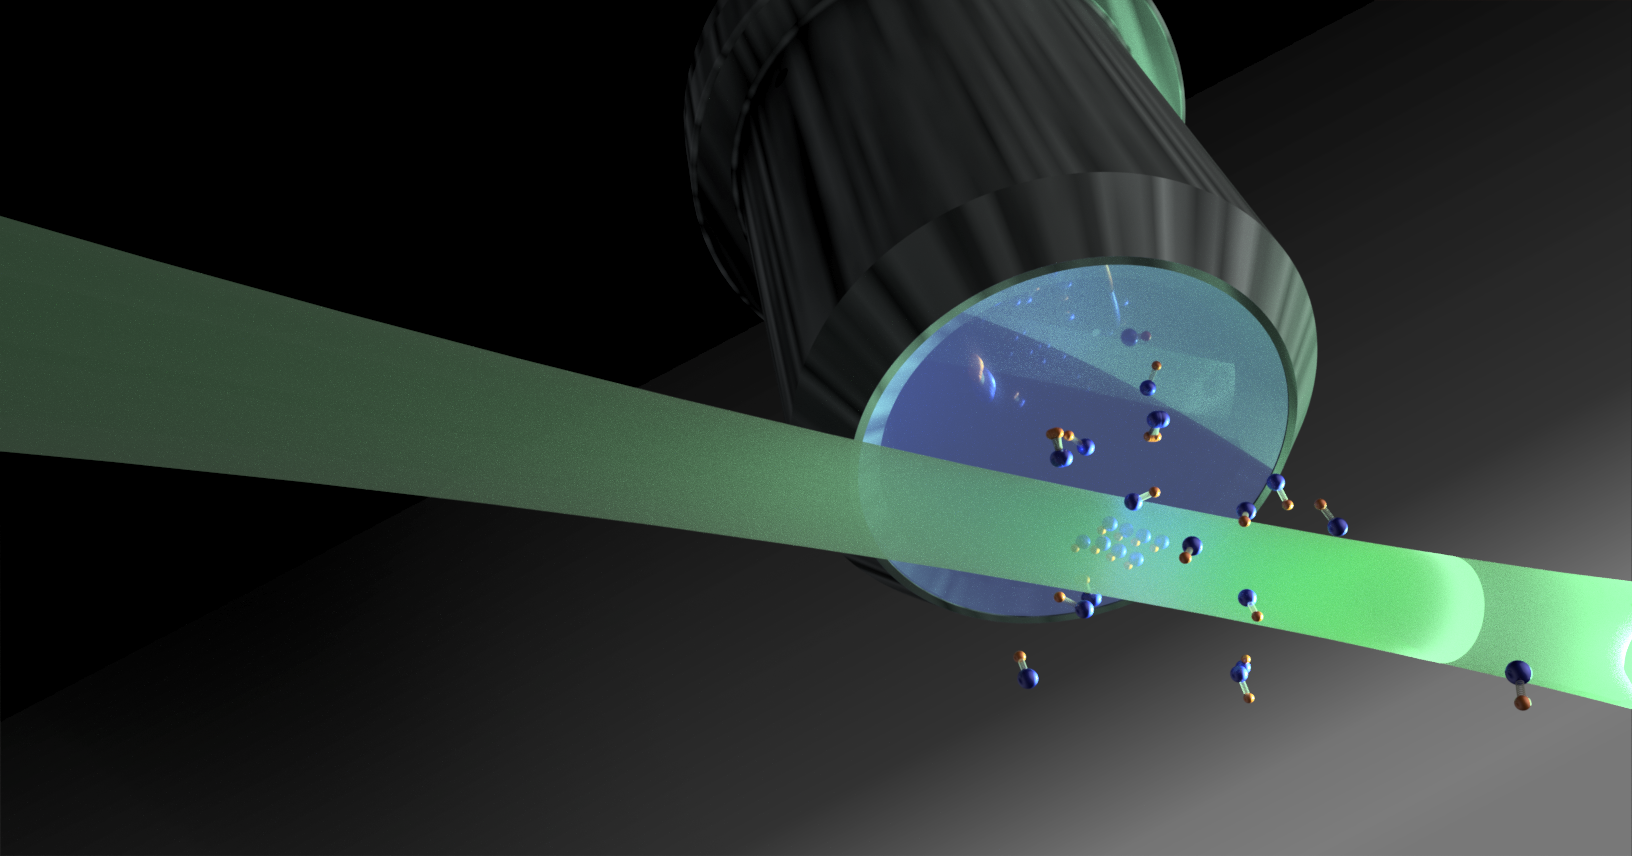
\includegraphics[height=\paperheight]{front_bg.png}}
    % 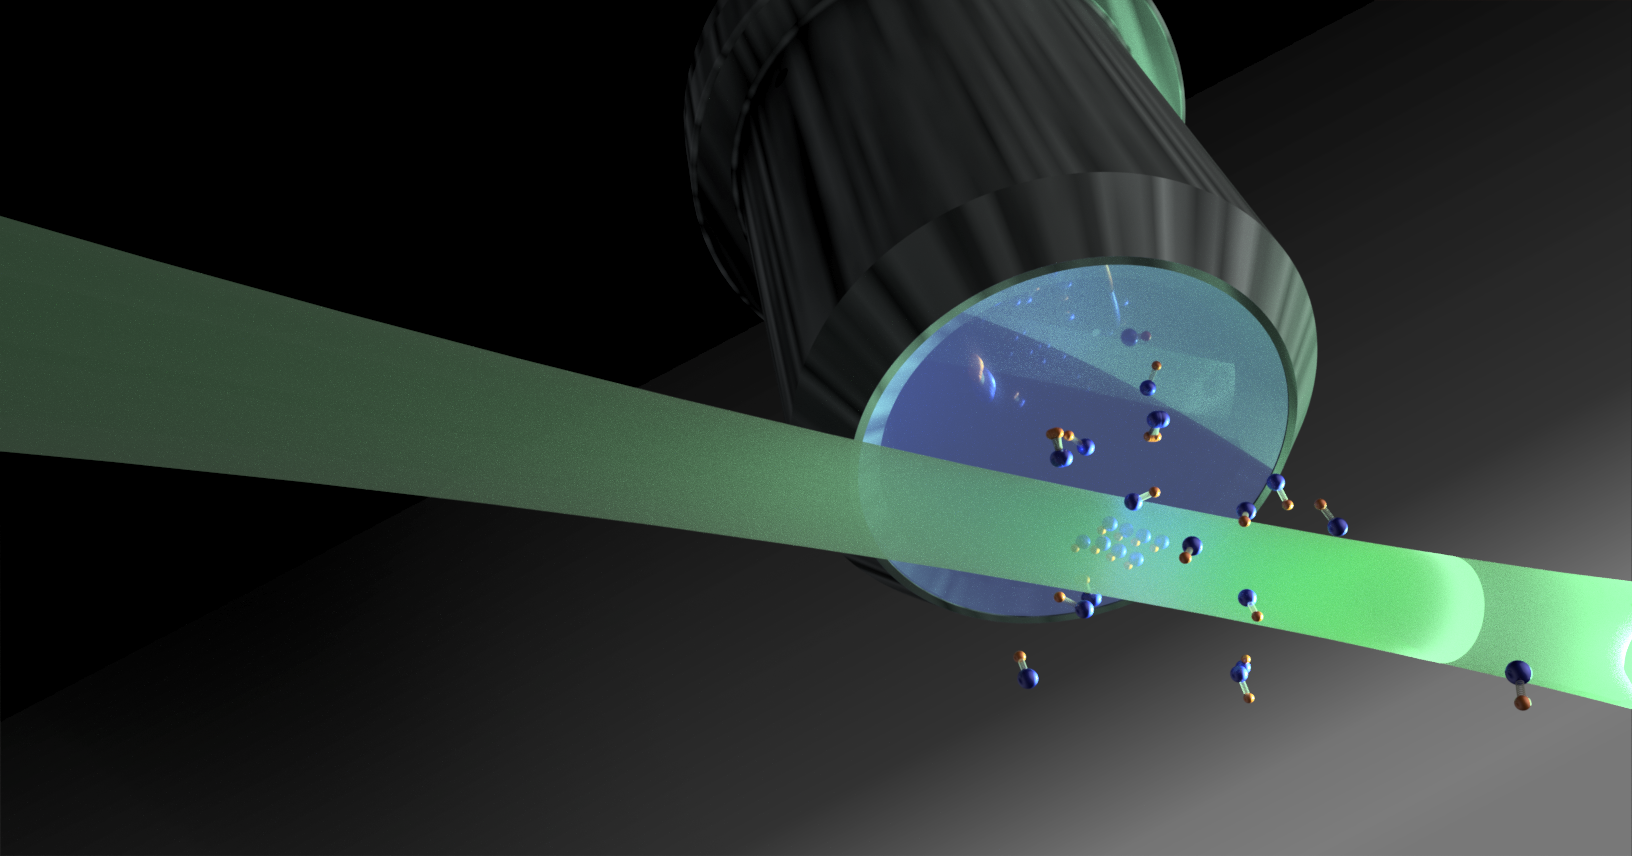
\includegraphics[height=\paperheight]{front_bg.png}
  }
  \setbeamercolor{title}{fg=cyan!30}
  \setbeamercolor{author}{fg=white}
  \setbeamercolor{institute}{fg=white}
  \setbeamercolor{date}{fg=white}
  \begin{frame}{}
    \titlepage
  \end{frame}
}

\pgfdeclarelayer{tweezer}
\pgfsetlayers{tweezer,main}
\pgfooclass{tweezer}{
  \method tweezer() {
  }
  \method drawTweezer(#1,#2,#3) {
    \begin{pgfonlayer}{tweezer}
      \shade[shading=radial,path fading=glow fading,shift={(#1,#2)},rotate=90,yscale=1,
      fill opacity=0.9,inner color=#3]
      plot[draw,samples=200,domain=-2.5:2.5] function {sqrt(0.01 + x**2 / 10)}
      -- plot[draw,samples=200,domain=2.5:-2.5] function {-sqrt(0.01 + x**2 / 10)};
    \end{pgfonlayer}
  }
  \method drawAtom(#1,#2,#3,#4) {
    \fill [#4,path fading=glow fading] (#1,#2) circle (#3);
  }
  \method drawNaAtom(#1,#2,#3) {
    \fill [blue,path fading=glow fading] (#1,#2) circle (#3);
  }
  \method drawCsAtom(#1,#2,#3) {
    \fill [red,path fading=glow fading] (#1,#2) circle (#3);
  }
  \method drawNaTweezer(#1,#2) {
    \pgfoothis.drawTweezer(#1,#2,green!50!orange);
  }
  \method drawCsTweezer(#1,#2) {
    \pgfoothis.drawTweezer(#1,#2,orange!50!yellow);
  }
  \method up(#1,#2) {
    \pgfoothis.drawCsTweezer(#1,#2);
    \pgfoothis.drawNaAtom(#1,#2+0.06,0.12);
    \pgfoothis.drawCsAtom(#1,#2-0.06,0.16);
  }
  \method down(#1,#2) {
    \pgfoothis.drawCsTweezer(#1,#2);
    \pgfoothis.drawCsAtom(#1,#2+0.06,0.16);
    \pgfoothis.drawNaAtom(#1,#2-0.06,0.12);
  }
  \method naTrap(#1,#2) {
    \pgfoothis.drawNaTweezer(#1,#2);
    \pgfoothis.drawNaAtom(#1,#2,0.12);
  }
  \method csTrap(#1,#2) {
    \pgfoothis.drawCsTweezer(#1,#2);
    \pgfoothis.drawCsAtom(#1,#2,0.16);
  }
}
\pgfoonew \mytweezer=new tweezer()
%%
% Array of trapped ultracold molecule
% * Strong and tunable interaction
% * Rich internal energy levels [READ-link: energy levels]
% * High filling
% * Single site detection
% * Single site manipulation
\begin{frame}{Molecules in optical tweezer}
  \begin{columns}
    \column{4.5cm}
    \begin{block}{Features}
      \begin{itemize}
      \item<2-> Strong and tunable interaction
      \item<3-> Rich internal energy levels
      \item<4-> High filling fraction
      \item<5-> Single site detection and manipulation
      \end{itemize}
    \end{block}
    \column{7cm}
    \begin{center}
      \begin{tikzpicture}[scale=0.9]
        \mytweezer.up(0, 0)
        \mytweezer.down(2, 0.8/2.5)
        \mytweezer.up(4, 1.2/2.5)
        \begin{pgfonlayer}{tweezer}
          \draw[line width=1,dashed,color=cyan] (0, 0/2.5) -- (2, 0.8/2.5);
          \draw[line width=1,dashed,color=cyan] (0, 0/2.5) -- (1, -1.7/2.5);
          \draw[line width=1,dashed,color=cyan] (2, 0.8/2.5) -- (1, -1.7/2.5);
          \draw[line width=1,dashed,color=cyan] (3, -2.1/2.5) -- (1, -1.7/2.5);
          \draw[line width=1,dashed,color=cyan] (3, -2.1/2.5) -- (2, 0.8/2.5);
          \draw[line width=1,dashed,color=cyan] (4, 1.2/2.5) -- (2, 0.8/2.5);
          \draw[line width=1,dashed,color=cyan] (3, -2.1/2.5) -- (4, 1.2/2.5);
          \draw[line width=1,dashed,color=cyan] (3, -2.1/2.5) -- (5, -1.9/2.5);
          \draw[line width=1,dashed,color=cyan] (4, 1.2/2.5) -- (5, -1.9/2.5);
          \draw[line width=1,dashed,color=cyan] (6.2, -0.9/2.5) -- (4, 1.2/2.5);
          \draw[line width=1,dashed,color=cyan] (6.2, -0.9/2.5) -- (5, -1.9/2.5);
        \end{pgfonlayer}
        \mytweezer.down(1, -1.7/2.5)
        \mytweezer.up(3, -2.1/2.5)
        \mytweezer.down(5, -1.9/2.5)
        \mytweezer.down(6.2, -0.9/2.5)
      \end{tikzpicture}
    \end{center}
  \end{columns}
\end{frame}

%%
% Like other ultracold atom and molecule toolboxs
% many applications
%
% Applications that are the most relevant
% * Quantum simulation [READ-link: simulation]
% * Quantum computation (digital simulation) [READ-link: quantum computation]
% {* Quantum chemistry}
% {* Test for fundamental physics}
\begin{frame}{Applications}
  \begin{block}{\only<1>{Simulation of many-body system\sfcite{Yan2013}}
      \only<2>{Quantum computation\sfcite{Yelin2006}}}
    \begin{center}
      \begin{tikzpicture}
        \visible<1>{
          \path (2.5, 0) node {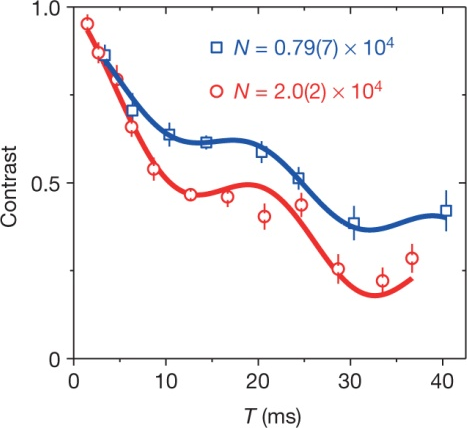
\includegraphics[width=4cm]{many-body-oscillation.png}};
          \path (-3.5, 0) node {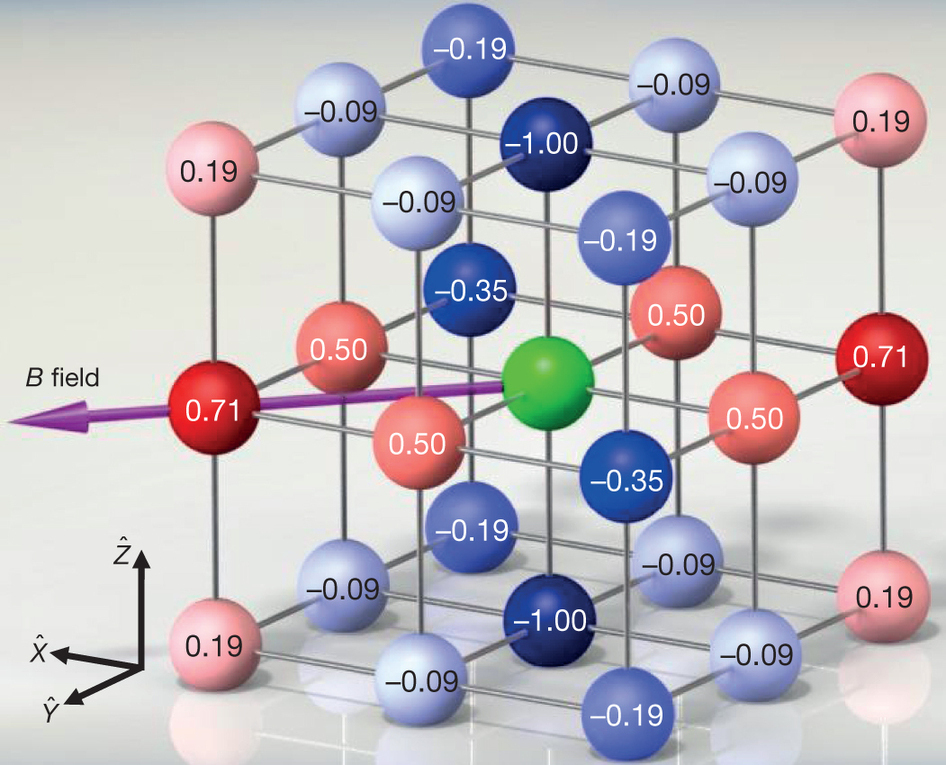
\includegraphics[width=7cm]{many-body-coupling.jpg}};
        }
        \visible<2>{
          \path (-1, 0) node {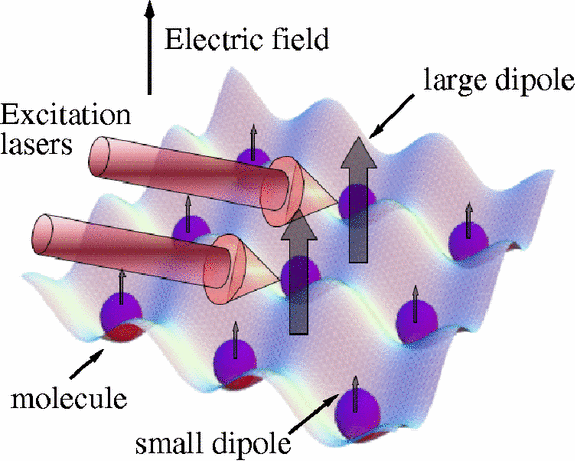
\includegraphics[width=7.5cm]{compute-geometry.png}};
        }
      \end{tikzpicture}
    \end{center}
  \end{block}
\end{frame}

%%
% * Use established atomic cooling techniques
%
% Experiment
% * MOT
% * Single atom
% * Cooling
% * Merging
% * Make molecule
\begin{frame}{Making molecules from atoms}
  \begin{columns}
    \column{4.5cm}
    \begin{itemize}
    \item<+-> MOT (Na + Cs)
    \item<+-> Loading single atoms \only<+->{}
    \item<+-> Raman sideband cooling
    \item<+-> Merge traps
    \item<+-> Make molecules!
    \end{itemize}
    \column{8cm}
    \begin{center}
      \begin{tikzpicture}
        \begin{pgfonlayer}{tweezer}
          \fill [opacity=0,white] (-3, -3) rectangle (3, 3);
        \end{pgfonlayer}
        \only<1-2>{
          \begin{pgfonlayer}{tweezer}
            \fill [red,fill opacity=0.2,path fading=glow fading] (-0.1,0) ellipse (2.5 and 1.5);
            \fill [blue,fill opacity=0.2,path fading=glow fading] (0.1,0) ellipse (2.5 and 1.5);
          \end{pgfonlayer}{tweezer}
        }
        \only<2-4>{
          \mytweezer.drawNaTweezer(0.6, 0.0)
          \mytweezer.drawCsTweezer(-0.6, 0.0)
        }
        \only<2-3>{
          \mytweezer.drawNaAtom(0.66, 0.05, 0.27)
          \mytweezer.drawCsAtom(-0.57, 0.04, 0.22)
        }
        \only<4>{
          \mytweezer.drawNaAtom(0.6, 0.0, 0.12)
          \mytweezer.drawCsAtom(-0.6, 0.0, 0.16)
        }
        \only<5>{
          \mytweezer.drawCsTweezer(0.0, 0.0)
          \mytweezer.drawNaAtom(0.06, 0.1, 0.12)
          \mytweezer.drawCsAtom(-0.04, -0.08, 0.16)
        }
        \only<6>{
          \mytweezer.up(0, 0)
        }
      \end{tikzpicture}
    \end{center}
  \end{columns}
\end{frame}

%%
% Current state
% * Cs more or less works as planned
\begin{frame}{Atom loading and cooling}
  \begin{columns}
    \column{5cm}
    \begin{itemize}
    \item<+-> Single atoms
    \item<+-> 85\% cround state after Cesium Raman sideband cooling
    \end{itemize}
    \column{6.5cm}
    \begin{center}
      \begin{tikzpicture}
        \visible<1>{
          \path (0, -2) node {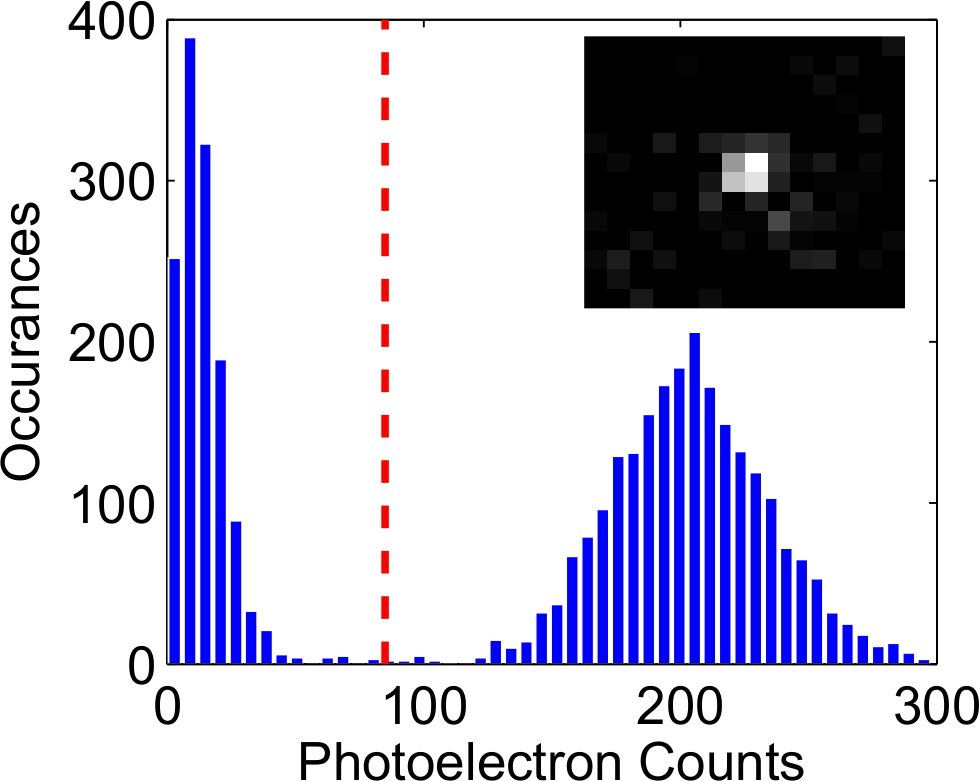
\includegraphics[width=6cm]{cs-histogram.png}};
          \path (0, 2) node
          {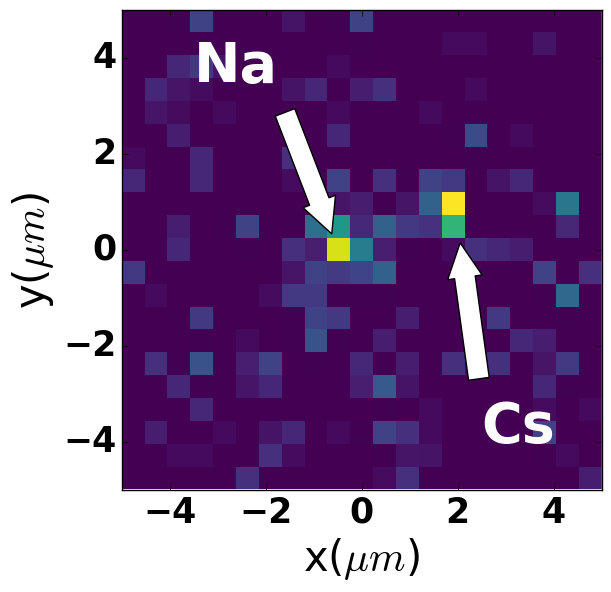
\includegraphics[width=3cm]{../../experiments/nacs_atoms/imgs/single_viridis.png}};
        }
        \visible<2>{
          \path (0, 0) node {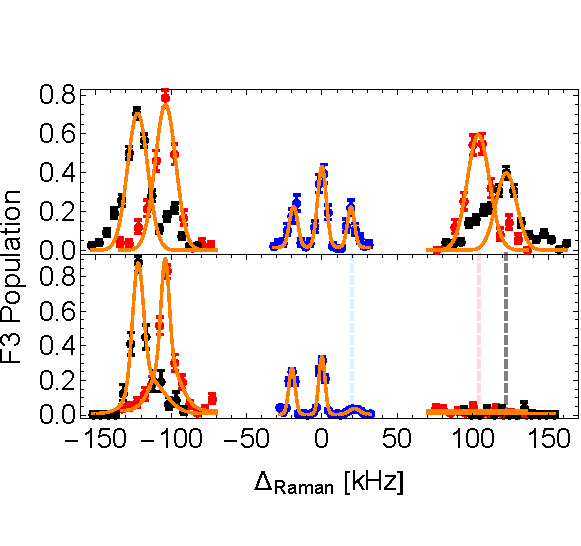
\includegraphics[width=6cm]{cs-raman-combined.pdf}};
        }
      \end{tikzpicture}
    \end{center}
  \end{columns}
\end{frame}

%%
% Na cooling
% [READ-link: excited state mixing due to strong lightshift (tensor lightshift)]
% * Challenges
% * Simulation
% * Result
\begin{frame}{Raman sideband cooling}
  \begin{columns}
    \column{6.5cm}
    \includegraphics[width=6cm]{Na_RSC_schematic.pdf}
    \column{5cm}
    \visible<2->{
      \begin{block}{Difficulties}
        \begin{itemize}
        \item High initial temperature ($40\mu K$)
        \item<3-> High recoil heating\\
          {\footnotesize (High Lamb Dicke parameter)}
        \end{itemize}
      \end{block}
    }
  \end{columns}
\end{frame}

\begin{frame}{Raman sidebands}
  \begin{center}
    \begin{tikzpicture}
      \visible<1> {
        \path (0, 0) node {
          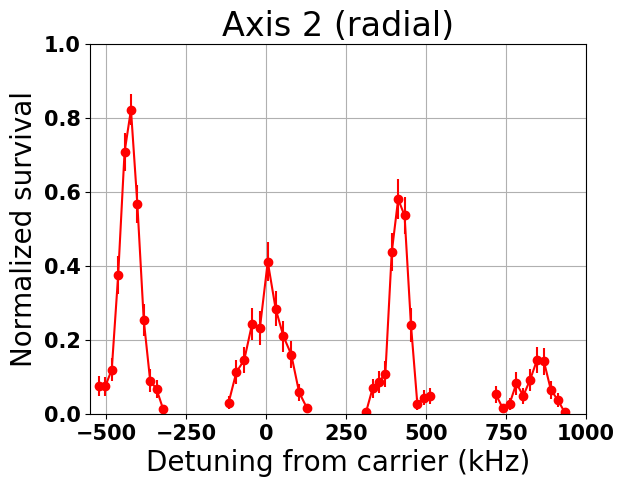
\includegraphics[width=10cm]{../../experiments/misc/imgs/data_spectrum_20170409_r2_before.png}
        };
        \draw[<-, line width=1.5] (-0.7, 0) -- (0, 1.6) node[right] {\Large Carrier};
      }
      \visible<2> {
        \path (0, 0) node {
          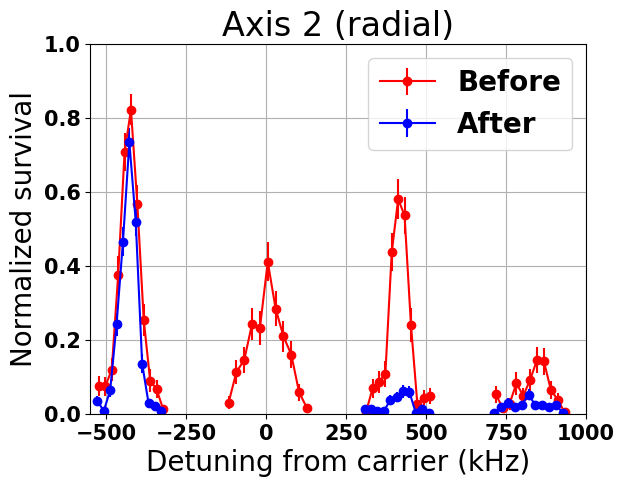
\includegraphics[width=10cm]{../../experiments/misc/imgs/data_spectrum_20170409_r2.png}
        };
      }
      \visible<3> {
        \path (0, 0) node {
          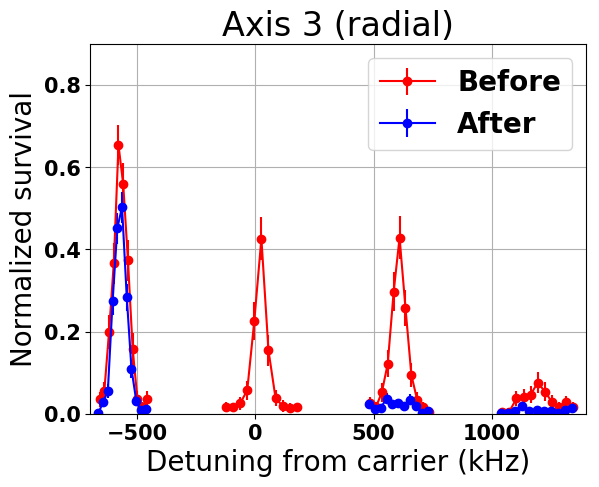
\includegraphics[width=10cm]{../../experiments/misc/imgs/data_spectrum_20170409_r3.png}
        };
      }
    \end{tikzpicture}
  \end{center}
\end{frame}

\begin{frame}{Raman sidebands}
  \begin{center}
    \begin{tikzpicture}[scale=1.41176]
      \visible<1> {
        \path (0, 0) node {
          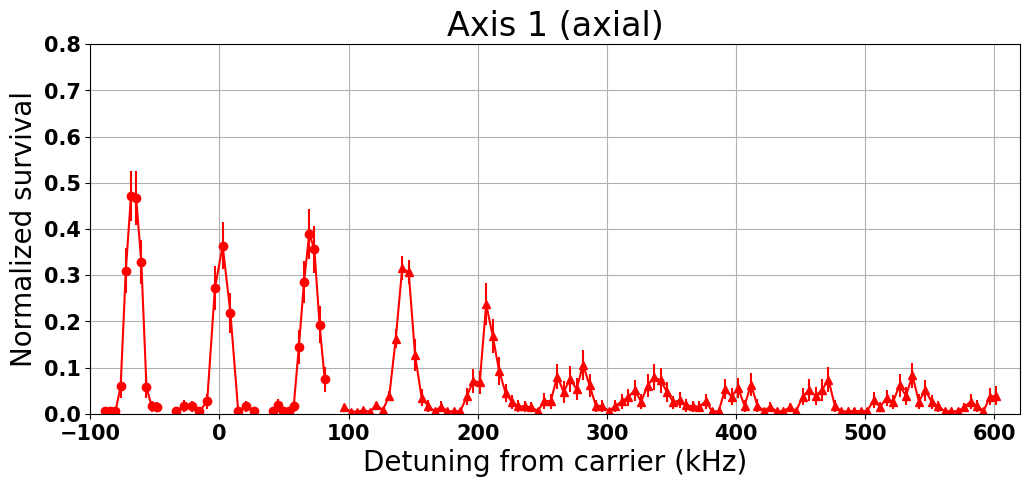
\includegraphics[width=12cm]{../../experiments/misc/imgs/data_spectrum_20170409_a1_before.png}
        };
        \draw[red, <-, line width=1.5] (-3.15, 0.5) -- (-2.95, 1.2)
        node[above right] {\Large 1st order heating};
        \draw[<-, line width=1.5] (-2.45, 0.2) -- (-2.25, 0.8) node[above right] {\Large Carrier};
        \draw[black!40!green, <-, line width=1.5] (-1.7, 0.2) -- (-1.55, 0.6)
        node[right] {\Large 1st order cooling};
        \draw[blue, <-, line width=1.5] (-0.95, -0.1) -- (-0.55, 0.1)
        node[right] {\Large 2nd order cooling};
        \path[magenta] (0.25, -0.5) node[right] {\Large And higher orders{$\cdots$}};
      }
      \visible<2-> {
        \path (0, 0) node {
          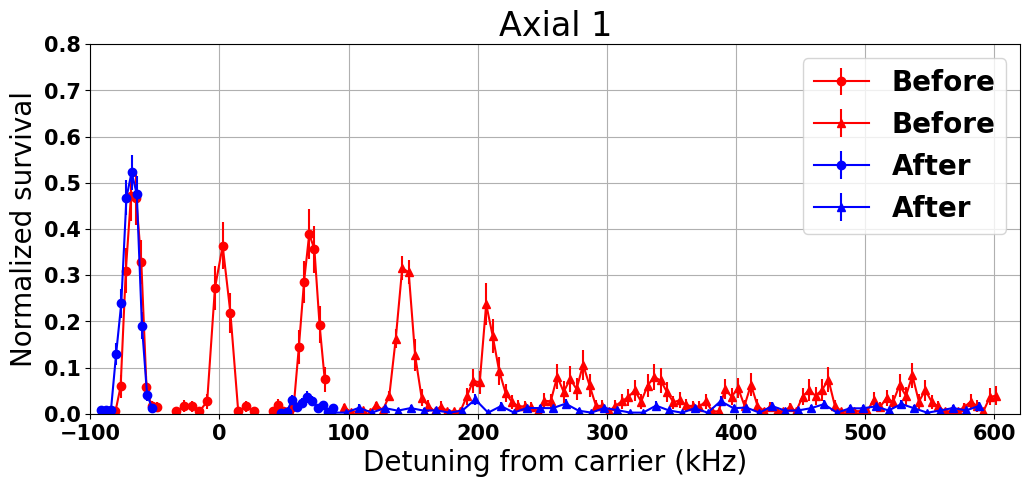
\includegraphics[width=12cm]{../../experiments/misc/imgs/data_spectrum_20170409_a1.png}
        };
      }
      \visible<3-> {
        \fill[white,opacity=0.95] (-4.2, -2.5) rectangle (5, 2.5);
        \path (0, 1) node[align=center]
        {
          \begin{tabular}{|c|c|}
            \hline
            \textbf{Axis}&\textbf{Ground state probability}\\\hline
            1 (Axial)&93.1(2.5)\%\\\hline
            2 (Radial)&91.9(2.3)\%\\\hline
            3 (Radial)&92.9(2.5)\%\\\hline
          \end{tabular}
        };
        \visible<4-> {
          \path (0, -1) node[align=center]
          {
            \textbf{3D ground state:} $79.5(3.6)\%$\\
            \textbf{Loss after cooling:} $15\%$\\\\
            \textbf{Total 3D ground state preparation fidelity:} $67.6(3.1)\%$
          };
        }
      }
    \end{tikzpicture}
  \end{center}
\end{frame}

\begin{frame}{Rabi flopping (radial)}
  \begin{center}
    \visible<+->{
      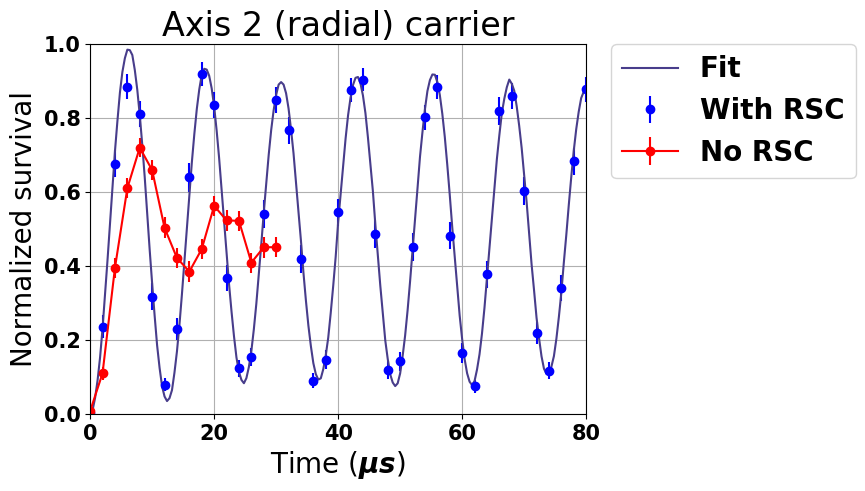
\includegraphics[width=10cm]{../../experiments/rabi_flop/imgs/fit_20170409_r2_0_ba.png}\\
    }
    \visible<+->{
      Good agreement in ground state probability between spectrum and Rabi flopping data.
    }
  \end{center}
\end{frame}

\begin{frame}{Rabi flopping (axial)}
  \begin{center}
    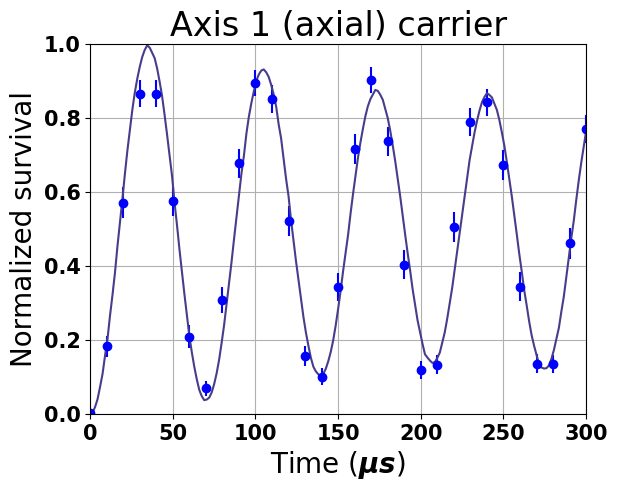
\includegraphics[height=4.8cm]{../../experiments/rabi_flop/imgs/fit_20170409_a1_0_nol.png}
    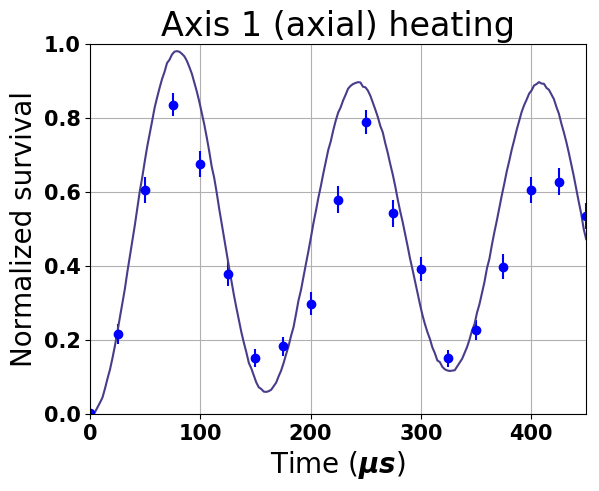
\includegraphics[height=4.8cm]{../../experiments/rabi_flop/imgs/fit_20170409_a1_p1_nol.png}
  \end{center}
\end{frame}

\begin{frame}{Axial matrix element}
  \begin{center}
    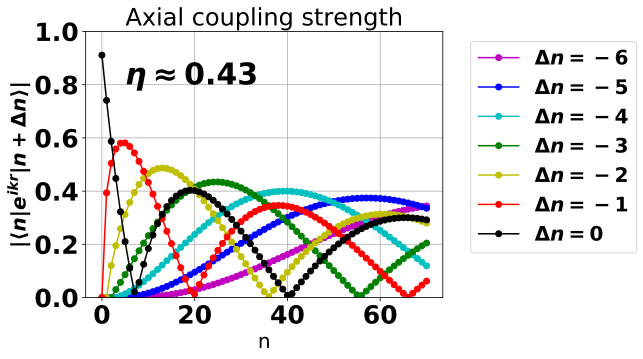
\includegraphics[width=6.5cm]{{../../calculations/sideband_strength/imgs/coupling_0.43_0-6}.png}
  \end{center}
\end{frame}

\begin{frame}{Radial 2 matrix element}
  \begin{center}
    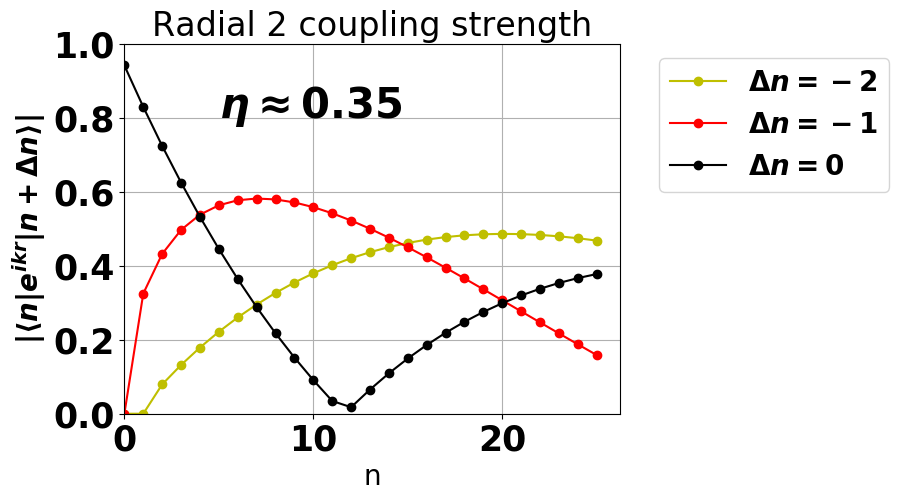
\includegraphics[width=6.5cm]{{../../calculations/sideband_strength/imgs/coupling_0.35_0-2}.png}
  \end{center}
\end{frame}

\begin{frame}{Radial 3 matrix element}
  \begin{center}
    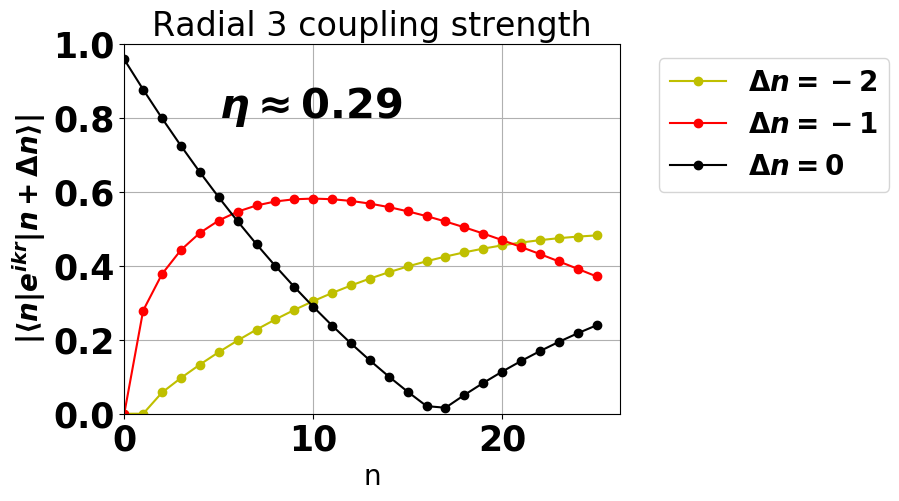
\includegraphics[width=6.5cm]{{../../calculations/sideband_strength/imgs/coupling_0.29_0-2}.png}
  \end{center}
\end{frame}

%%
% Next step
% * Merge
% * Transfer
\begin{frame}{Next step}
\end{frame}

\begin{frame}{}
\end{frame}

\end{document}
